\documentclass[aspectratio=169]{beamer}

% ------------------------------------------------------------
% Minimal Yachay Tech style - LaTeX Beamer
% Project: Respiratory Sound Anomaly Classification
% Sections included: 1 to 6 only. Metrics/results are excluded.
% ------------------------------------------------------------

\usepackage[utf8]{inputenc}
\usepackage[T1]{fontenc}
\usepackage{lmodern}
\usepackage{booktabs}
\usepackage{array}
\usepackage{tabularx}
\usepackage{graphicx}
\usepackage{xcolor}
\usepackage{tikz}
\usetikzlibrary{arrows.meta, positioning, shapes.geometric}

\definecolor{YachayBlue}{HTML}{005B9A}
\definecolor{SoftGray}{HTML}{F2F4F7}
\definecolor{DarkGray}{HTML}{333333}

\setbeamertemplate{navigation symbols}{}
\setbeamertemplate{footline}[frame number]
\setbeamertemplate{headline}{%
  \begin{beamercolorbox}[wd=\paperwidth,ht=0.35cm,dp=0.05cm]{headline}
    \colorbox{YachayBlue}{\hspace{\paperwidth}\vspace{0.28cm}}
  \end{beamercolorbox}%
}

\setbeamercolor{title}{fg=black}
\setbeamercolor{frametitle}{fg=black}
\setbeamercolor{normal text}{fg=black,bg=white}
\setbeamerfont{frametitle}{series=\bfseries,size=\Large}
\setbeamerfont{title}{series=\bfseries,size=\LARGE}

\newcommand{\important}[1]{\textcolor{YachayBlue}{\textbf{#1}}}
\newcommand{\smallsource}[1]{\vspace{0.15cm}{\scriptsize\color{DarkGray}#1}}

\title{Respiratory Sound Anomaly Classification}
\subtitle{Artificial Intelligence Project}
\author{Juan Fernando Cevallos Bravo}
\institute{Yachay Tech University}
\date{2026}

\begin{document}

% ------------------------------------------------------------
\begin{frame}
  \titlepage
  \vspace{-0.2cm}
  \centering
  \important{Biomedical AI} for respiratory sound analysis using classical machine learning.
\end{frame}

% ------------------------------------------------------------
\begin{frame}{1. Topic and Objectives}
\textbf{Project topic:} Detection of \important{abnormal respiratory cycles} from lung sounds.

\vspace{0.35cm}
\textbf{Problem to solve:} respiratory sounds can contain acoustic signs such as \important{crackles} and \important{wheezes}, but manual auscultation depends on clinical experience and may be difficult to standardize.

\vspace{0.35cm}
\textbf{Specific objectives:}
\begin{itemize}
    \item Segment each recording into respiratory cycles using the official \important{.txt annotations}.
    \item Extract interpretable acoustic features from every cycle: \important{MFCC, RMS, ZCR, spectral centroid, bandwidth and rolloff}.
    \item Train and compare two classifiers: \important{Logistic Regression} and \important{Random Forest}.
\end{itemize}
\end{frame}

% ------------------------------------------------------------
\begin{frame}{Acoustic Features Used by the Model}
\small

\textbf{Goal:} each respiratory cycle is transformed into a compact numerical representation. 
These values are \textcolor{blue}{not fixed diagnostic thresholds}; they are patterns learned by the model.

\vspace{0.25cm}

\begin{table}
\centering
\renewcommand{\arraystretch}{1.25}
\begin{tabular}{p{2.6cm} p{4.0cm} p{4.1cm}}
\hline
\textbf{Feature} & \textbf{What it describes} & \textbf{Model interpretation} \\
\hline
\textcolor{blue}{MFCC} & Spectral texture & General acoustic shape of the cycle \\
\textcolor{blue}{RMS} & Signal energy & Higher amplitude means stronger acoustic activity \\
\textcolor{blue}{ZCR} & Zero crossings & High values suggest rapid changes or noisy patterns \\
\textcolor{blue}{Centroid} & Frequency center & Shows if energy is low- or high-frequency dominated \\
\textcolor{blue}{Bandwidth} & Frequency spread & Measures dispersion around the spectral centroid \\
\textcolor{blue}{Rolloff} & Energy limit & Frequency below which most energy is concentrated \\
\hline
\end{tabular}
\end{table}

\vspace{0.15cm}

\footnotesize
The official anomaly label comes from the annotation file: 
\textcolor{blue}{$crackles=1$ or $wheezes=1$}.

\end{frame}
\begin{frame}{1. Objective Reformulation}
\textbf{Main objective:}

\vspace{0.3cm}
Classify respiratory cycles according to the \important{presence or absence of acoustic anomalies}, using features extracted from segmented audio signals.

\vspace{0.4cm}
\begin{block}{Target definition}
\centering
\important{Normal} = crackles 0 and wheezes 0

\important{Anomaly} = crackles 1 or wheezes 1
\end{block}

\vspace{0.25cm}
This project does not directly diagnose COPD, asthma or pneumonia; it detects \important{cycle-level acoustic abnormalities} that may be clinically associated with respiratory disease.
\end{frame}

% ------------------------------------------------------------
\begin{frame}{2. State of the Art: Deep Learning Approaches}
\scriptsize
\renewcommand{\arraystretch}{1.25}
\begin{tabularx}{\textwidth}{>{\raggedright\arraybackslash}p{2.0cm} >{\raggedright\arraybackslash}X >{\raggedright\arraybackslash}p{2.1cm} >{\raggedright\arraybackslash}p{2.2cm}}
\toprule
\textbf{Author / Year} & \textbf{Dataset} & \textbf{Model} & \textbf{Main result} \\
\midrule
Petmezas et al. & ICBHI 2017 & Hybrid \important{CNN-LSTM} & Accuracy 73.69; ICBHI Score 64.92 \\
Nguyen et al. & ICBHI 2017 & \important{ResNet50} co-tuning & ICBHI Score 58.29 in 4 classes \\
Yang et al. & ICBHI 2017 & ResNet + GoogLeNet + attention & ICBHI Score \important{72.72} \\
Bae et al. & ICBHI 2017 & Audio Spectrogram Transformer & Patch-Mix contrastive learning \\
Wanasinghe et al. & ICBHI + Mendeley & Lightweight CNN & Accuracy up to \important{91.04} \\
\bottomrule
\end{tabularx}

\smallsource{These studies show that spectrogram-based deep learning is powerful, but requires more computation, careful tuning and longer experimental time.}
\end{frame}

% ------------------------------------------------------------
\begin{frame}{2. State of the Art: Alternative Models and Features}
\scriptsize
\renewcommand{\arraystretch}{1.25}
\begin{tabularx}{\textwidth}{>{\raggedright\arraybackslash}p{2.0cm} >{\raggedright\arraybackslash}X >{\raggedright\arraybackslash}p{2.2cm} >{\raggedright\arraybackslash}p{2.2cm}}
\toprule
\textbf{Author / Year} & \textbf{Dataset} & \textbf{Model} & \textbf{Main result} \\
\midrule
Zhang et al. & ICBHI 2017 & Dual-channel \important{CNN-LSTM} & Accuracy 99.01, recall 99.13 \\
Gupta et al. & 6-class lung sounds & DeepRespNet 1D / 2D & Accuracy \important{95.2} with 2D \\
Xiao et al. & ICBHI 2017 & AST + LungAdapter & 2-class ICBHI Score 69.53 \\
Tzeng et al. & ICBHI + FABS & Audio enhancement + CNN/AST & Better robustness with enhancement \\
Zhang et al. & 112 subjects & \important{ANN with 15 acoustic features} & Test accuracy 94; external 90 \\
\bottomrule
\end{tabularx}

\smallsource{For a fast and rigorous university project, feature-based classical ML is more realistic than a full transfer learning pipeline.}
\end{frame}

% ------------------------------------------------------------
\begin{frame}{2. Comparative Decision}
\small
\renewcommand{\arraystretch}{1.3}
\begin{tabularx}{\textwidth}{>{\bfseries}p{3.2cm} X X}
\toprule
\textbf{Approach} & \textbf{Advantage} & \textbf{Limitation} \\
\midrule
Transfer Learning CNN & Strong performance on spectrogram images & Requires image generation, GPU, tuning and longer time \\
CNN from scratch & Biomedical deep learning pipeline & Risk of overfitting and slow iteration \\
\important{Logistic Regression} & Interpretable, fast, rigorous baseline & Linear decision boundary \\
\important{Random Forest} & Nonlinear classifier, robust to feature interactions & Less interpretable than logistic regression \\
\bottomrule
\end{tabularx}

\vspace{0.35cm}
\centering
\important{Final decision:} binary classification using acoustic features, Logistic Regression and Random Forest.
\end{frame}

% ------------------------------------------------------------
\begin{frame}{3. Pipeline}
\centering
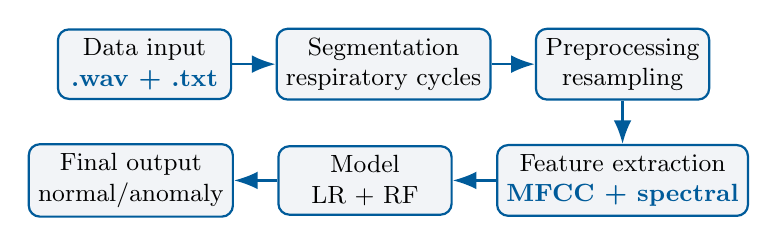
\begin{tikzpicture}[
    node distance=0.55cm,
    box/.style={rectangle, rounded corners, draw=YachayBlue, thick, fill=SoftGray, minimum width=2.2cm, minimum height=0.8cm, align=center, font=\small},
    arrow/.style={-{Latex[length=3mm]}, thick, color=YachayBlue}
]

\node[box] (input) {Data input\\\important{.wav + .txt}};
\node[box, right=of input] (seg) {Segmentation\\respiratory cycles};
\node[box, right=of seg] (prep) {Preprocessing\\resampling};
\node[box, below=of prep] (feat) {Feature extraction\\\important{MFCC + spectral}};
\node[box, left=of feat] (model) {Model\\LR + RF};
\node[box, left=of model] (output) {Final output\\normal/anomaly};

\draw[arrow] (input) -- (seg);
\draw[arrow] (seg) -- (prep);
\draw[arrow] (prep) -- (feat);
\draw[arrow] (feat) -- (model);
\draw[arrow] (model) -- (output);

\end{tikzpicture}

\vspace{0.45cm}
\small
The system transforms raw biomedical audio into \important{structured numerical features}, then predicts whether each respiratory cycle is normal or abnormal.
\end{frame}

% ------------------------------------------------------------
\begin{frame}{4. Database}
\small
\renewcommand{\arraystretch}{1.3}
\begin{tabularx}{\textwidth}{>{\bfseries}p{3.0cm} X}
\toprule
Dataset name & Respiratory Sound Database, Kaggle version: \important{vbookshelf/respiratory-sound-database} \\
Source & KaggleHub download inside Google Colab \\
Samples & \important{920 audio files} and \important{6,898 annotated respiratory cycles} \\
Subjects & \important{126 patients} with different ages and respiratory conditions \\
Biomedical data type & Respiratory audio signals recorded with digital stethoscopes \\
Classes from .txt & Normal, crackles, wheezes and both \\
Clinical metadata & COPD, asthma, pneumonia, healthy and other diagnoses may appear in CSV metadata \\
\bottomrule
\end{tabularx}
\end{frame}

% ------------------------------------------------------------
\begin{frame}{4. Data Structure}
\small
\begin{columns}[T]
\column{0.48\textwidth}
\textbf{Annotation files (.txt)}
\begin{itemize}
    \item Start time of the cycle
    \item End time of the cycle
    \item \important{Crackles: 0 or 1}
    \item \important{Wheezes: 0 or 1}
\end{itemize}

\column{0.48\textwidth}
\textbf{Audio files (.wav)}
\begin{itemize}
    \item Raw respiratory sound signal
    \item Variable duration
    \item Variable sampling rate
    \item Requires \important{resampling to 4000 Hz}
\end{itemize}
\end{columns}

\vspace{0.35cm}
\begin{block}{Machine learning unit}
\centering
\important{One row in .txt = one respiratory cycle = one sample}
\end{block}
\end{frame}

% ------------------------------------------------------------
\begin{frame}{4. Example Sample Definition}
\small
\renewcommand{\arraystretch}{1.25}
\begin{tabular}{ccccc}
\toprule
\textbf{Start} & \textbf{End} & \textbf{Crackles} & \textbf{Wheezes} & \textbf{Label} \\
\midrule
0.036 & 1.207 & 0 & 0 & \important{Normal} \\
1.207 & 3.450 & 1 & 0 & \important{Crackles} \\
3.450 & 5.800 & 0 & 1 & \important{Wheezes} \\
5.800 & 8.100 & 1 & 1 & \important{Both} \\
\bottomrule
\end{tabular}

\vspace{0.45cm}
For the final simplified model, the multiclass labels are converted into a binary target:

\vspace{0.15cm}
\centering
\important{0 = normal} \hspace{0.8cm} \important{1 = acoustic anomaly}
\end{frame}

% ------------------------------------------------------------
\begin{frame}{5. Model}
\small
\textbf{Selected architecture:} classical supervised machine learning with \important{Logistic Regression} as the main model and \important{Random Forest} as comparison.

\vspace{0.3cm}
\textbf{Why this model was selected:}
\begin{itemize}
    \item It is compatible with a feature table extracted from biomedical audio.
    \item It is faster and safer than transfer learning for the available time.
    \item Logistic Regression provides an \important{interpretable baseline}.
    \item Random Forest captures \important{nonlinear acoustic patterns}.
\end{itemize}

\vspace{0.15cm}
\textbf{Input:} one vector of acoustic features per respiratory cycle.
\end{frame}

% ------------------------------------------------------------
\begin{frame}{5. Feature Extraction}
\small
\renewcommand{\arraystretch}{1.25}
\begin{tabularx}{\textwidth}{>{\bfseries}p{3.0cm} X}
\toprule
Feature group & Purpose \\
\midrule
\important{MFCC mean/std} & Captures the spectral texture of respiratory sounds \\
RMS energy & Measures signal intensity within the cycle \\
Zero crossing rate & Captures fast waveform variation and acoustic roughness \\
Spectral centroid & Indicates where the center of spectral energy is located \\
Spectral bandwidth & Measures spectral spread \\
Spectral rolloff & Identifies frequency concentration of most signal energy \\
Duration & Adds cycle-level physiological timing information \\
\bottomrule
\end{tabularx}

\vspace{0.25cm}
These features convert each audio cycle into a \important{numerical vector} suitable for classical ML.
\end{frame}

% ------------------------------------------------------------
\begin{frame}{5. Main Parameters}
\small
\renewcommand{\arraystretch}{1.25}
\begin{tabularx}{\textwidth}{>{\bfseries}p{3.2cm} X}
\toprule
Component & Parameter decision \\
\midrule
Sampling rate & \important{4000 Hz} for all audio cycles \\
Target task & Binary classification: normal vs anomaly \\
Train/test split & Group split by \important{patient ID} to avoid data leakage \\
Logistic Regression & StandardScaler + LogisticRegression, max\_iter = 1000, class\_weight = balanced \\
Random Forest & n\_estimators = 300, class\_weight = balanced, random\_state = 42 \\
Optimizer / epochs & Not applicable; these models are not neural networks \\
Learning rate / batch size & Not applicable for Logistic Regression and Random Forest in scikit-learn \\
\bottomrule
\end{tabularx}
\end{frame}

% ------------------------------------------------------------
\begin{frame}{6. Flowchart}
\centering
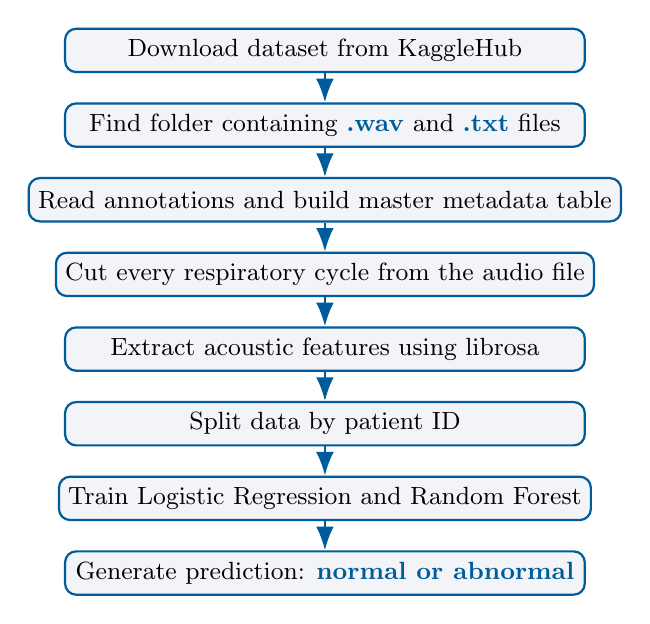
\begin{tikzpicture}[
    node distance=0.37cm,
    box/.style={rectangle, rounded corners, draw=YachayBlue, thick, fill=SoftGray, minimum width=6.6cm, minimum height=0.55cm, align=center, font=\small},
    arrow/.style={-{Latex[length=3mm]}, thick, color=YachayBlue}
]

\node[box] (a) {Download dataset from KaggleHub};
\node[box, below=of a] (b) {Find folder containing \important{.wav} and \important{.txt} files};
\node[box, below=of b] (c) {Read annotations and build master metadata table};
\node[box, below=of c] (d) {Cut every respiratory cycle from the audio file};
\node[box, below=of d] (e) {Extract acoustic features using librosa};
\node[box, below=of e] (f) {Split data by patient ID};
\node[box, below=of f] (g) {Train Logistic Regression and Random Forest};
\node[box, below=of g] (h) {Generate prediction: \important{normal or abnormal}};

\foreach \i/\j in {a/b,b/c,c/d,d/e,e/f,f/g,g/h}{\draw[arrow] (\i) -- (\j);}

\end{tikzpicture}
\end{frame}

% ------------------------------------------------------------
\begin{frame}{References for State of the Art}
\tiny
\begin{enumerate}
    \item G. Petmezas et al., Automated lung sound classification using a hybrid CNN-LSTM network and focal loss function.
    \item T.-T. Nguyen et al., Lung sound classification using co-tuning and stochastic normalization.
    \item Z. Yang et al., Respiratory sound classification by applying deep neural network with a blocking variable.
    \item S. H. Bae et al., Patch-Mix contrastive learning with audio spectrogram transformer on respiratory sound classification.
    \item T. Wanasinghe et al., Lung sound classification with multi-feature integration utilizing lightweight CNN model.
    \item Y. Zhang et al., Lung sound classification model based on dual-channel CNN-LSTM algorithm.
    \item R. Gupta et al., DeepRespNet: A deep neural network for classification of respiratory sounds.
    \item L. Xiao et al., LungAdapter: Efficient adapting audio spectrogram transformer for lung sound classification.
    \item J.-T. Tzeng et al., Improving robustness and clinical applicability of respiratory sound classification using audio enhancement.
    \item W. Zhang et al., High-accuracy lung sound classification for healthy versus unhealthy diagnosis using ANN.
\end{enumerate}

\vspace{0.2cm}
\important{Note:} Metrics and final results slides are intentionally excluded until the model is executed.
\end{frame}

slide del diagrama de mel comparativo 
\begin{frame}{Mel-Diagram}
    
\begin{figure}
    \centering
    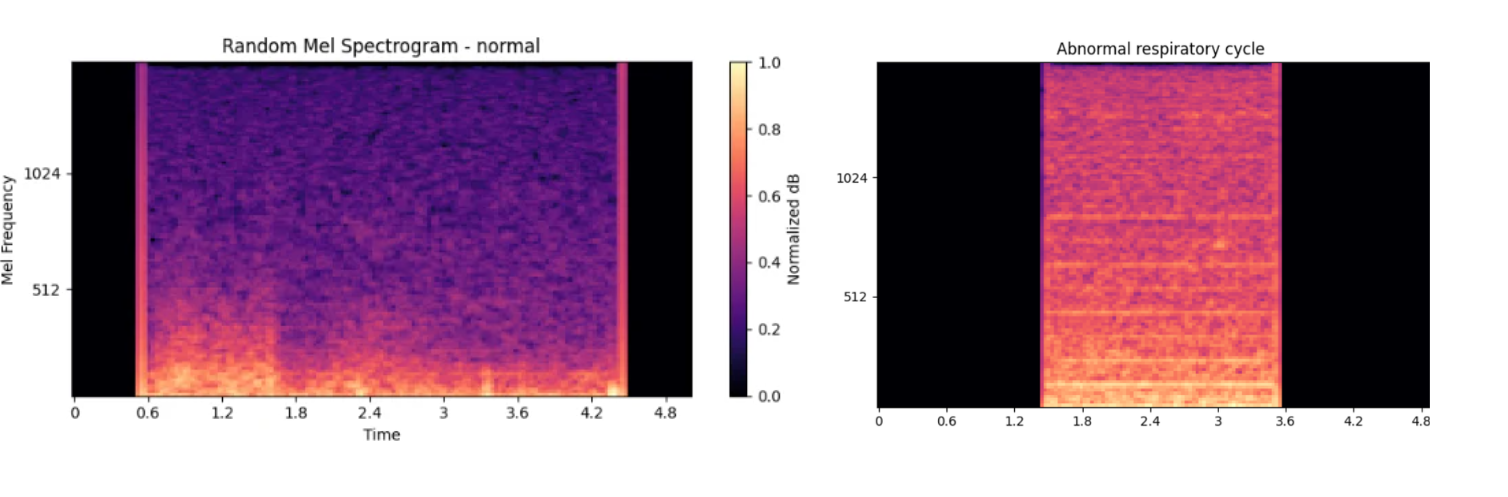
\includegraphics[width=0.85\linewidth]{image02.png}
    \caption{MEL}
    \label{fig:placeholder}
\end{figure}
\end{frame}
% =========================
% MODEL METRICS
% =========================

\begin{frame}{Model Metrics Comparison}
\small

The models were evaluated using \textcolor{blue}{Accuracy}, \textcolor{blue}{Precision}, \textcolor{blue}{Recall}, \textcolor{blue}{F1-score}, and \textcolor{blue}{ROC-AUC}. These metrics compare the real labels from the annotation files with the predicted labels.

\vspace{0.2cm}

\begin{center}
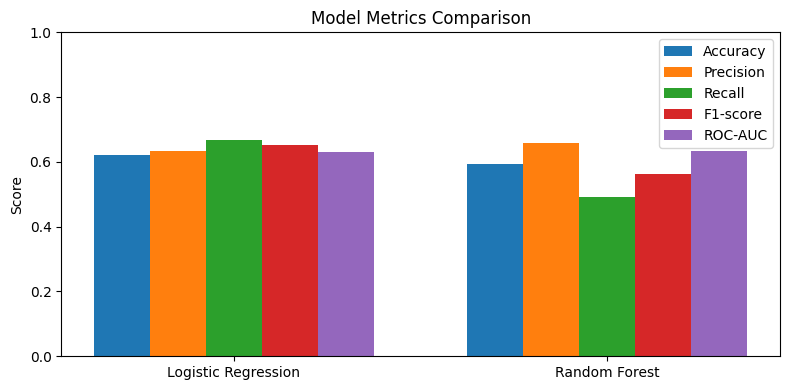
\includegraphics[width=0.82\textwidth]{modelm.png}
\end{center}

\vspace{0.1cm}
\footnotesize
Caption: Performance comparison between \textcolor{blue}{Logistic Regression} and \textcolor{blue}{Random Forest}.

\end{frame}


% =========================
% CONFUSION MATRIX
% =========================

\begin{frame}{Confusion Matrix}
\small

The confusion matrix shows the number of cycles classified as \textcolor{blue}{normal} or \textcolor{blue}{abnormal}. The diagonal values represent correct predictions, while the off-diagonal values represent errors.

\vspace{0.2cm}

\begin{center}
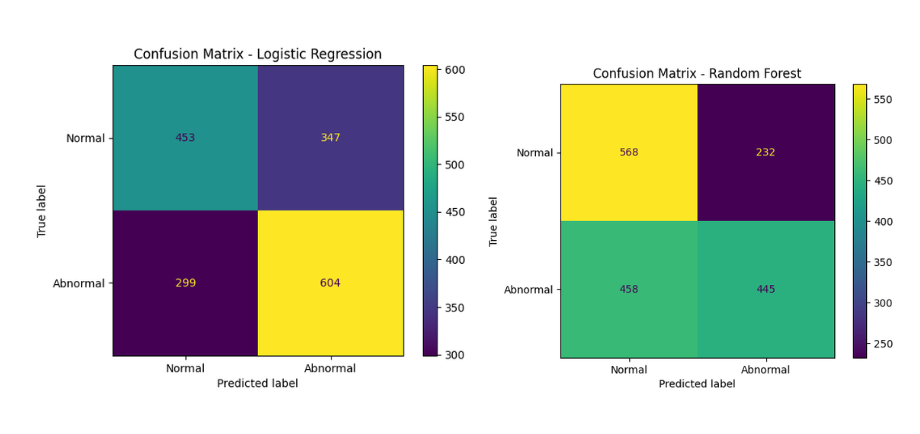
\includegraphics[width=0.88\textwidth]{confusion.png}
\end{center}

\vspace{0.1cm}
\footnotesize
Caption: Logistic Regression detected more abnormal cycles, while Random Forest classified more normal cycles correctly.

\end{frame}


% =========================
% ROC CURVES
% =========================

\begin{frame}{ROC Curves}
\small

ROC curves show the ability of each model to separate \textcolor{blue}{normal} and \textcolor{blue}{abnormal} respiratory cycles across different classification thresholds.

\vspace{0.2cm}

\begin{columns}
\column{0.39\textwidth}
\centering
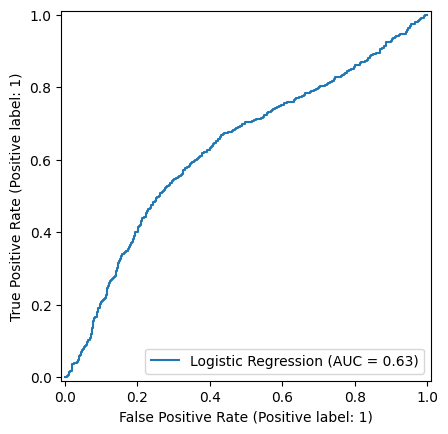
\includegraphics[width=\textwidth]{roc1.png}

\column{0.39\textwidth}
\centering
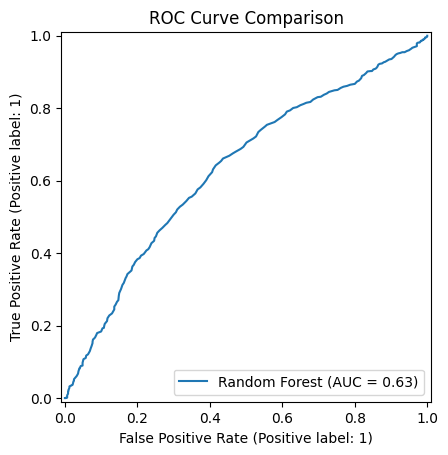
\includegraphics[width=\textwidth]{roc2.png}
\end{columns}

\vspace{0.1cm}
\footnotesize
Caption: ROC curves for Logistic Regression and Random Forest.

\end{frame}


% =========================
% FEATURE IMPORTANCE
% =========================

\begin{frame}{Feature Importance}
\small

Random Forest was used to identify the acoustic features with the greatest contribution to the classification. This helps interpret which signal descriptors were more relevant for detecting \textcolor{blue}{respiratory anomalies}.

\vspace{0.2cm}

\begin{center}
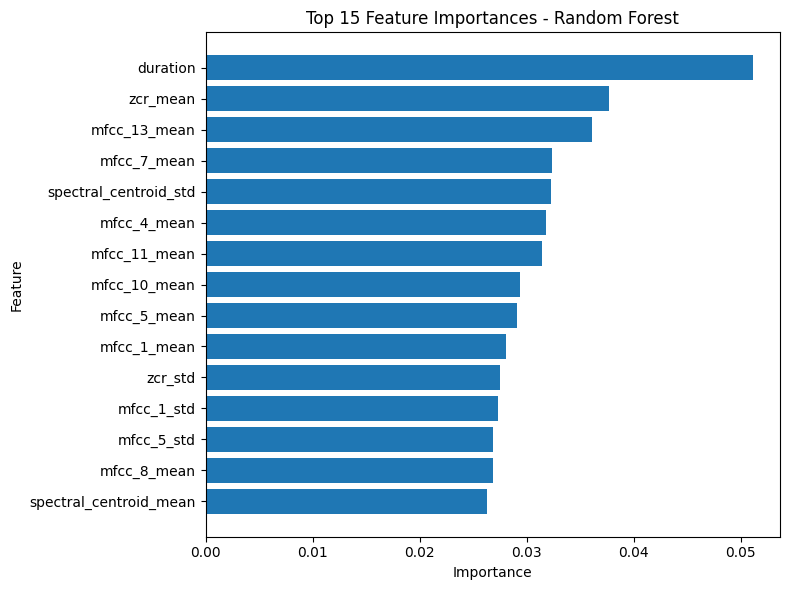
\includegraphics[width=0.52\textwidth]{importance.png}
\end{center}

\vspace{0.1cm}
\footnotesize
Caption: Most relevant acoustic features for classifying normal and abnormal respiratory cycles.

\end{frame}

\end{document}

